\documentclass[../main.tex]{subfiles}

\begin{document}
	\newcommand{\pe}[1]{\hat{\underline #1}}
	\section{Stabilit\'a e punti di equilibrio}
		Finora abbiamo parlato di stabilit\'a mettendo in relazione ingresso e uscita. Adesso introduciamo un nuovo concetto di stabilit\'a che mette in relazione stato e controllo.
		
	\subsection{Definizione qualitativa}
		Si dice \textbf{punto di equilibrio} una configurazione in cui il sistema si trova e dopo una piccola perturbazione rimane in questa configurazione.
		
		Consideriamo qualche esempio pratico per definire i possibili punti di equilibrio:
		\begin{figure}[H]
			\centering
			\begin{subfigure}{0.24\textwidth}
				\includegraphics[width=\linewidth]{punto_equilibrio/casoA}
				\caption{asintoticamente stabile}
				\label{fig:asint_stab}
			\end{subfigure}
			$\;\;\;\;\;\;$
			\centering
			\begin{subfigure}{0.24\textwidth}
				\includegraphics[width=\linewidth]{punto_equilibrio/casoB}
				\caption{instabile}
				\label{fig:instabile}
			\end{subfigure}
			$\;\;\;\;\;\;$
			\centering
			\begin{subfigure}{0.24\textwidth}
				\includegraphics[width=\linewidth]{punto_equilibrio/casoC}
				\caption{semplicemente stabile}
				\label{fig:sempl_stab}
			\end{subfigure}
			\caption{}
		\end{figure}
	
		\begin{itemize}
			\item
				\ref{fig:asint_stab}: \'e un punto di equilibrio \textbf{asintoticamente stabile} perch\'e se perturbo leggermente la posizione della pallina, essa torna subito nel suo punto di equilibrio. Inoltre \'e un p.e. \textbf{isolato} perch\'e non ci sono altri p.e. nelle vicinanze;
			\item
				\ref{fig:instabile}: \'e un punto di equilibrio \textbf{instabile} perch\'e se muovo leggermente la pallina, essa si allontana indefinitamente dal p.e.;
			\item
				\ref{fig:sempl_stab}: \'e un punto di equilibrio \textbf{semplicemente stabile} perch\'e se perturbo la posizione della pallina essa trova un nuovo punto di equilibrio. Inoltre \'e un p.e. \textbf{non isolato} perch\'e nelle vicinanze ci sono altri p.e.
		\end{itemize}
		I punti di equilibrio non isolati non possono essere asintoticamente stabili perch\'e il sistema pu\'o trovare un nuovo punto di equilibrio in un intorno del precedente.
		
	\subsection{Definizione}
		Consideriamo l'equazione di stato di un generico sistema non lineare:
		\begin{align*}
			\underline{\dot x}(t) &= \underline f(\underline x(t), \underline u(t))\\
			\underline y(t) &= \underline g(\underline x(t), \underline u(t))
		\end{align*}
		Una coppia stato-controllo $ \hat P = (\pe x, \pe u) \in \R $ \'e punto di equilibrio \textbf{se e solo se} $ \underline f (\pe x, \pe u) = 0 $ (cio\'e la derivata dello stato \'e nulla $ \underline{\dot x}(t) = 0 $).
		
	\subsubsection*{Esempio}
		Consideriamo il sistema non lineare della vasca di cui avevamo parlato nell'introduzione. La sua equazione di stato era:
		\[ \dot h(t) = -\frac{E}{S} \sqrt{2g h(t)} + \frac{1}{S} u(t) \]
		I punti di equilibrio sono:
		\[ \forall (h, u)\ \text{t.c.}\ -\frac{E}{S} \sqrt{2g h(t)} + \frac{u}{S} = 0 \]
		\begin{equation}
			\label{es_condizione_pe}
			\Rightarrow \hat u = E \sqrt{2g \hat h}
		\end{equation}
		
		Cerchiamo di capire la tipologia di questo punto di equilibrio e per questo fissiamo l'ingresso (l'acqua fornita dal rubinetto) al valore di equilibrio $ u(t) = \hat u $:
		\begin{itemize}
			\item se aggiungiamo acqua dall'esterno superando il livello di equilibrio $ h(t) > \hat h $, dalla condizione di punto di equilibrio \ref{es_condizione_pe} otteniamo che $ E \sqrt{2gh(t)} > \hat u $. Allora dall'equazione di stato ricaviamo $ S \dot h(t) = \hat u - E \sqrt{2gh(t)} < 0 $, la derivata \'e negativa, cio\'e che il livello dell'acqua scende tornando subito al punto di equilibrio $ (\hat u, \hat h) $;
			\item se togliamo dell'acqua dalla vasca $ h(t) < \hat h $, allora $ \dot h(t) > 0 $, cio\'e il livello risale tornando al punto di equilibrio di partenza $ (\hat u, \hat h) $.
		\end{itemize}
		Deduciamo che si tratta di un punto di equilibrio asintoticamente stabile.
		
	\subsection{Studio della stabilit\'a dei punti di equilibrio per sistemi lineari}
		In generale in un sistema non \'e detto che i punti di equilibrio siano tutti dello stesso tipo.
		Noi adesso consideriamo l'equazione di stato di un sistema lineare:
		\[ \dot{\underline{x}}(t) = A \underline x(t) + B\underline u(t) \]
		non consideriamo la seconda equazione perch\'e siamo interessati solo alla stabilit\'a dello stato.\\
		Prendiamo un punto di equilibrio $ (\pe x, \pe u) $, quindi per definizione $ A \pe x + B \pe u = 0 $. Definisco:
		\begin{align}
			\delta \underline x(t) &= \underline x(t) - \pe x \qquad \text{scostamento di \underline x rispetto al particolare}\ \pe x\\
			\dot{\delta \underline x}(t) &= \der{}{t} (\underline x(t) - \pe x)
			\label{eq:def}
		\end{align}
		
		Consideriamo l'equazione di stato quando viene applicato $ \underline u = \pe u $: $ \dot{\underline{x}}(t) = A \underline x(t) + B\underline{\hat u} $ e calcolata nel punto di equilibrio: $ \dot{\hat{\underline{x}}} = A \underline{\hat x} + B\underline{\hat u} $ quindi sottraiamo membro a membro:
		\begin{align*}
			\dot{\underline{x}}(t) - \dot{\pe x} &= A (\underline x(t) - \pe x) + B(\pe u - \pe u)\\
			\der{}{t} (\underline x(t) - \pe x) &= A (\underline x(t) - \pe x)
		\end{align*}
		In base alle definizioni \ref{eq:def} otteniamo:
		\begin{equation}
			\dot{\delta \underline x}(t) = A \delta \underline x(t)
			\label{eq:evoluzione_scostamento}
		\end{equation}
		cio\'e $ \delta \underline x(t) $ evolve con equazioni pari a quelle di $ \underline x(t) $ in assenza di controllo.
		
		Per fare questi calcoli siamo partiti da un particolare punto di equilibrio, ma in \ref{eq:evoluzione_scostamento} questa dipendenza si \'e persa perci\'o \ref{eq:evoluzione_scostamento} vale $ \forall (\pe x, \pe u) $. Quindi se abbiamo la stessa evoluzione di $ \delta x(t) $ per ogni p.e., questo significa che \underline{per i sistemi lineari tutti i punti di equilibrio sono dello stesso tipo}. Si parla quindi di stabilit\'a del sistema (riferendosi al tipo di stabilit\'a comune a tutti i suoi p.e.). Allora per semplicit\'a scelgo $ (0,0) $ che \'e sempre punto di equilibrio. 
		
		In definitiva studiare la stabilit\'a di tutti i punti di equilibrio corrisponde allo studiare la stabilit\'a dell'evoluzione libero dello stato:
		\begin{align*}
			\underline x_l(t) = e^{At} \underline x(0^-)
			X_l(s) = (sI-A)^{-1} \underline x(0^-)
		\end{align*}
		
	\subsection{Stabilit\'a di un sistema}
		Un sistema \'e stabile oppure instabile a seconda di come si comporta $ \vec x_l(t) $.\\
		Un sistema lineare tempo invariante \'e:
		\begin{itemize}
			\item
				\textbf{asintoticamente stabile} $ \Leftrightarrow  \forall \underline x(0^-)\ \text{tale che}\ \underline x_l(t) $ non diverge e $ \underline x_l(t) \xrightarrow[t \rightarrow \infty]{} 0 $;
			\item
				\textbf{instabile} $ \Leftrightarrow  \forall \underline x(0^-)\ \text{tale che}\ \underline x_l(t) $ diverge;
			\item
				\textbf{semplicemente stabile} $ \Leftrightarrow $ non \'e verificata nessuna delle condizioni precedenti, cio\'e
				\begin{align*}
					&\nexists\ \underline x(0^-)\ \text{tale che}\ \underline x_l(t)\ \text{diverga}\\
					&\exists\ \underline x(0^-)\ \text{tale che}\ \underline x_l(t)\ \text{non tende a zero}
				\end{align*}
		\end{itemize}
	
	\subsubsection*{Esempio}
		\begin{equation*}
			\dot x = \matThree{1}{0}{0}{0}{-1}{0}{0}{0}{0} x + Bu
		\end{equation*}
		Il termine $ Bu $ non \'e utile ai fini del calcolo della stabilit\'a, ma lo mettiamo per completezza.
		\[ 
			\begin{cases}
				\dot x_1 &= x_1\\
				\dot x_2 &= -x_2\\
				\dot x_3 &= 0
			\end{cases}
		\]
		L'evoluzione libera della stato (la soluzione di queste equazioni differenziali) \'e:
		\[ 
			x_l(t) = 
			\begin{cases}
				x_{1l} &= e^t x_1(0^-)\\
				x_{2l} &= e^{-t} x_2(0^-)\\
				x_{3l} &= x_3(0^-)
			\end{cases}
			\quad = e^{At} \underline x(0^-) = \matThree{e^t}{0}{0}{0}{e^{-t}}{0}{0}{0}{1} \underline x(0^-)
		\]
		  
		Adesso studiamo la stabilit\'a del sistema dati alcuni stati iniziali:
		\begin{enumerate}
			\item
				\[ \underline x(0^-) = \begin{bmatrix} 3\\ 0\\ 0 \end{bmatrix} \quad \Rightarrow \quad x_l(t) = \begin{bmatrix} 3e^t\\ 0\\ 0 \end{bmatrix} \]
				Abbiamo trovato uno stato iniziale $ \underline x(0^-) $ per cui l'evoluzione libera diverge. Quindi il base alla definizione precedente possiamo stabilire che il sistema \'e instabile.
			\item
				\[ \underline x(0^-) = \begin{bmatrix} 0\\ 0\\ 5 \end{bmatrix} \quad \Rightarrow \quad x_l(t) = \begin{bmatrix} 0\\ 0\\ 5 \end{bmatrix} \]
				In questo caso lo stato rimane limitato ma non tende a zero.
			\item
				\[ \underline x(0^-) = \begin{bmatrix} 0\\ -2\\ 0 \end{bmatrix} \quad \Rightarrow \quad x_l(t) = \begin{bmatrix} 0\\ -2e^{-t}\\ 0 \end{bmatrix} \]
				In questa particolare situazione, lo stato tende a zero.                
		\end{enumerate}                                                           
	                                                                           
	\subsection{Studio della stabilit\'a attraverso $ e^{At} $}       
		\begin{itemize}                                                           
			\item                                                                    
				\textbf{asintoticamente stabile} $ \Leftrightarrow $ tutte le componenti di $ e^{At} $ sono segnali $ \xrightarrow[t \rightarrow \infty]{} 0 $;
			\item
				\textbf{instabile} $ \Leftrightarrow $ esiste una componente di $ e^{At} $ che sia un segnale divergente;
			\item
				\textbf{semplicemente stabile} $ \Leftrightarrow $ non esistono componenti di $ e^{At} $ divergenti, ma esiste almeno una componente che sia un segnale semplicemente stabile (limitato ma che non tende a zero).
		\end{itemize}
		
		Poich\'e gli elementi di $ (sI-A)^{-1} $ sono le trasformate di Laplace dei corrispondenti elementi di $ e^{At} $, il sistema \'e:
		\begin{itemize}
			\item
				\textbf{asintoticamente stabile} $ \Leftrightarrow $ tutte le radici di ogni denominatore degli elementi di $ (sI-A)^{-1} $ sono a $ \Re < 0 $;
			\item
				\textbf{instabile} $ \Leftrightarrow $ esiste un elemento di $ (sI-A)^{-1} $, il cui denominatore ha almeno una radice a $ \Re > 0 $ oppure almeno una radice $ \Re = 0 $ con molteplicit\'a $ > 1 $;
			\item
				\textbf{semplicemente stabile} $ \Leftrightarrow $ non esistono radici di nessun denominatore a $ \Re > 0 $ oppure esiste almeno una radice a $ \Re = 0 $ e tutte hanno molteplicit\'a 1.
		\end{itemize}
	
	\subsubsection*{Esempio}
		\[ \dot x =
			\begin{bmatrix}
				1 & 0 & 0\\
				0 & -1 & 0\\
				0 & 0 & 0
			\end{bmatrix} x
		\]
		\[ (sI-A)^{-1} =
			\begin{bmatrix}
				s-1 & 0 & 0\\
				0 & s+1 & 0\\
				0 & 0 & 0
			\end{bmatrix}^{-1} =
			\begin{bmatrix}
				\frac{1}{s-1} & 0 & 0\\
				0 & \frac{1}{s+1} & 0\\
				0 & 0 & \frac{1}{s}
			\end{bmatrix}
		\]
		Il primo termini della matrice ha una radice a $ \Re > 0 $ quindi il sistema \'e instabile.
		
	\subsubsection*{Esempio}
	\label{esempio:semplicemente_stabile}
		\[ \dot x =
			\begin{bmatrix}
				0 & 0\\
				0 & 0
			\end{bmatrix} x = \begin{bmatrix} 0\\ 0 \end{bmatrix}
		\]
		Qualunque stato iniziale \'e punto di equilibrio per il sistema, che quindi non possono essere isolati. Questo sistema allora non pu\'o essere asintoticamente stabile.
		\[ e^{At} =
			\begin{bmatrix} e^{0t} & 0\\ 0 & e^{0t} \end{bmatrix} =
			\begin{bmatrix} 1 & 0\\ 0 & 1\\ \end{bmatrix} \qquad
			(sI-A)^{-1} = \begin{bmatrix} \frac{1}{s} & 0\\ 0 & \frac{1}{s} \end{bmatrix}
		\]
		Le radici del denominatore sono tutte a $ \Re = 0 $ con molteplicit\'a 1. Allora il sistema \'e semplicemente stabile.
		
	\subsubsection*{Esempio}
		\[ 
			\dot x = \begin{bmatrix} 0 & 1\\ 0 & 0 \end{bmatrix} x
		\]
		\[
			(sI-A)^{-1} = \begin{bmatrix} s & -1\\ 0 & s \end{bmatrix} = \begin{bmatrix} \frac{1}{s} & \frac{1}{s^2}\\ 0 & \frac{1}{s} \end{bmatrix}
		\]
		Il sistema \'e instabile perch\'e esiste una radice con molteplicit\'a 2.
		
	\subsection{Studio della stabilit\'a attraverso il polinomio minimo}
		Un sistema \'e:
		\begin{itemize}
			\item
				\textbf{asintoticamente stabile} se tutte le radici di $ m(s) $ hanno $ \Re < 0 $;
			\item
				\textbf{instabile} se $ m(s) $ ha almeno una radice a $ \Re > 0 $ oppure esiste almeno una radice a $ \Re = 0 $ ma tutte con molteplicit\'a $ >1 $ in $ m(s) $;
			\item
				\textbf{semplicemente stabile} in tutte le altre situazioni: nessuna radice a $ \Re > 0 $ e esiste almeno una radice a $ \Re = 0 $ con molteplicit\'a $ =1 $ in $ m(s) $.
		\end{itemize}
	
	\subsubsection*{Esempio}
		\[
			\dot x=
			\begin{tikzpicture}[baseline=-0.5ex]
				\matrix [matrix of math nodes,left delimiter={[},right delimiter={]}] (m)
				{
					1 & \phantom{-} 0 	& \phantom{-} 0 	& \phantom{-} 2 \\               
					0 & -1 				& \phantom{-} 1 	& \phantom{-} 3 \\               
					0 & \phantom{-} 0 	& \phantom{-} 0 	& \phantom{-} 1 \\
					0 & \phantom{-} 0 	& -1 				& \phantom{-} 0 \\           
				};  
				\draw[color=red] (m-1-1.north west) -- (m-1-1.north east) -- (m-1-1.south east) -- (m-1-1.south west) -- (m-1-1.north west);
				\draw[color=red] (m-2-2.north west) -- (m-2-2.north east) -- (m-2-2.south east) -- (m-2-2.south west) -- (m-2-2.north west);
				\draw[color=red] (m-3-3.north west) -- (m-3-4.north east) -- (m-4-4.south east) -- (m-4-3.south west) -- (m-3-3.north west);
			\end{tikzpicture} x
		\]
		Si tratta di una matrice triangolare a blocchi: gli autovalori sono l'unione degli autovalori delle sottomatrici.\\
		\[
			\phi(s) = det
			\begin{bmatrix}
				s-1	& 0		& 0		& -2\\
				0	& s+1	& -1	& -3\\
				0	& 0		& s		& -1\\
				0	& 0		& 1		& s
			\end{bmatrix}
			= (s-1)(s+1)(s^2+1)
		\]
		Abbiamo 4 autovalori distinti: 1, -1, j, -j. Il sistema \'e instabile a causa di 1 perch\'e ha $ \Re > 0 $.
		
	\subsubsection*{Esempio}
		\[
			\dot x=
			\begin{tikzpicture}[baseline=-0.5ex]
				\matrix [matrix of math nodes,left delimiter={[},right delimiter={]}] (m)
				{
					-1	& \phantom{-} 1 	& \phantom{-} 3 	& \phantom{-} 5 \\               
					0	& -1 				& \phantom{-} 7 	& \phantom{-} 9 \\               
					0	& \phantom{-} 0 	& \phantom{-} 0 	& \phantom{-} 0 \\
					0	& \phantom{-} 0 	& \phantom{-} 1 	& \phantom{-} 0 \\           
				};  
				\draw[color=red] (m-1-1.north west) -- (m-1-1.north east) -- (m-1-1.south east) -- (m-1-1.south west) -- (m-1-1.north west);
				\draw[color=red] (m-2-2.north west) -- (m-2-2.north east) -- (m-2-2.south east) -- (m-2-2.south west) -- (m-2-2.north west);
				\draw[color=red] (m-3-3.north west) -- (m-3-4.north east) -- (m-4-4.south east) -- (m-4-3.south west) -- (m-3-3.north west);
			\end{tikzpicture} x
		\]
		Si tratta di una matrice a blocchi. Inoltre il "blocco" $ 2 \times 2 $ \'e triangolare quindi gli autovalori sono gli elementi sulla diagonale. Gli autovalori della matrice sono: -1, -1, 0, 0.
		\[ \phi(s) = (s+1)^2 s^2 \]
		In questo caso il polinomio caratteristico mi dice solo che il sistema non \'e asintoticamente stabile perch\'e \'e presente una radice a $ \Re = 0 $ con molteplicit\'a 2. Allora studio $ (sI-A)^{-1} $.
		\[
			(sI-A)^{-1} =
			\begin{bmatrix}
				s+1	& *		& *		& *\\
				0	& s+1	& *		& *\\
				0	& 0		& s		& 0\\
				0	& 0		& -1	& s\\
			\end{bmatrix}^{-1}
		\]
		Con $ * $ indichiamo i valori restanti della matrice che per ora non ci servono.\\
		I primi due blocchi $ 1 \times 1 $ della matrice si invertono e otteniamo $ \frac{1}{s+1} $. Il terzo blocco $ 2 \times 2 $ lo calcoliamo a parte:
		\[
			\begin{bmatrix}
				s	& 0\\[5pt]
				-1	& s
			\end{bmatrix}^{-1} =
			\begin{bmatrix}
				\frac{1}{s}		& 0\\[5pt]
				\frac{1}{s^2}	& \frac{1}{s}
			\end{bmatrix}
		\]
		Il (2,1)-esimo elemento denota la instabilit\'a perch\'e mi assicura che anche nel polinomio minimo \'e presente il termine $ s^2 $ (cio\'e una radice a $ \Re = 0 $, con molteplicit\'a 2). Se non avessi trovato questo termine, avrei dovuto calcolare anche i termini della matrice inversa corrispondenti agli $ * $.
		
	\subsubsection*{Esempio}
		Al contrario del precedente, in questo esercizio non ci baster\'a fare l\'inversa degli elementi sulla diagonale, ma dovremmo calcolare anche i restanti.
		\[
			\dot x=
			\begin{tikzpicture}[baseline=-0.5ex]
			\matrix [matrix of math nodes,left delimiter={[},right delimiter={]}] (m)
			{
				\phantom{-} 0	& \phantom{-} 1 	& \phantom{-} 0 	& \phantom{-} 0 \\               
				-1				& \phantom{-} 0 	& \phantom{-} 1 	& \phantom{-} 0 \\               
				\phantom{-} 0	& \phantom{-} 0 	& \phantom{-} 0 	& -1 \\
				\phantom{-} 0	& \phantom{-} 0 	& \phantom{-} 1 	& \phantom{-} 0 \\           
			};  
			\draw[color=red] (m-1-1.north west) -- (m-1-2.north east) -- (m-2-2.south east) -- (m-2-1.south west) -- (m-1-1.north west);
			\draw[color=red] (m-3-3.north west) -- (m-3-4.north east) -- (m-4-4.south east) -- (m-4-3.south west) -- (m-3-3.north west);
			\end{tikzpicture} x
		\]
		\'E una matrice triangolare a blocchi, quindi gli autovalori sono l'unione degli autovalori di ogni blocco. Per entrambi i blocchi gli autovalori sono $ \pm j $, quindi avremo che gli autovalori della matrice sono j e -j con molteplicit\'a 2. Allora il polinomio caratteristico \'e:
		\[ \phi(s) = (s^2+1)^2 \]
		Deduciamo subito che il sistema non pu\'o essere asintoticamente stabile perch\'e sono presenti radici a $ \Re = 0 $. Per determinare la stabilit\'a studiamo $ (sI-A)^{-1} $.\\
		Facciamo l'inversa rispettivamente del primo e del secondo blocco:
		\[
			\begin{bmatrix}
				s & -1\\[5pt]
				1 & s
			\end{bmatrix}^{-1} = 
			\begin{bmatrix}
				\frac{s}{s^+1} & \frac{1}{s^+1}\\[5pt]
				-\frac{1}{s^+1} & \frac{s}{s^+1}
			\end{bmatrix}
		\]
		\[
			\begin{bmatrix}
				s & 1\\[5pt]
				-1 & s
			\end{bmatrix}^{-1} =
			\begin{bmatrix}
				\frac{s}{s^+1} & -\frac{1}{s^+1}\\[5pt]
				\frac{1}{s^+1} & \frac{s}{s^+1}
			\end{bmatrix}
		\]
		Guardando solo questi blocchi concluderei erroneamente che il sistema \'e semplicemente stabile perch\'e nel polinomio minimo abbiamo un fattore $ s^2+1 $, invece di $ (s^2+1)^2 $, quindi esiste una radice a $ \Re = 0 $ con molteplicit\'a 1. In realt\'a basta calcolare l'inversa di un elemento non sulla diagonale, ad esempio il (1,3)-esimo:
		\[ (sI-A)^{-1}_{1,3} = \frac{s}{(s^+1)^2} \]
		Possiamo anche non calcolare i restanti elementi dell'inversa, perch\'e questo appena calcolato ci assicura che nel polinomio minimo \'e presente il termine $ (s^2+1)^2 $, quindi c'\'e una radice a $ \Re=0 $ con molteplicit\'a 2.\\
		Il sistema \'e instabile.
		
	\subsection{Linearizzazione dei sistemi non lineari}
		Considero il seguente sistema
		\begin{equation*}
			\dot x(t) = f \left[ x(t), u(t) \right]
		\end{equation*}
		dove $ f $ \'e una funzione non lineare.\\
		Considero il punto di equilibrio $ \hat P=(\hat x, \hat u) $, quindi per definizione di p.e. $ f(\hat x, \hat u) = 0 $.\\
		Definiamo:
		\begin{align*}
			\delta x(t) &= x(t) - \hat x\\
			\delta u(t) &= u(t) - \hat u
		\end{align*}
		Scriviamo il polinomio di Taylor di $ f $ attorno $ (\hat x, \hat u) $:
		\begin{align*}
			\dot{\delta x}(t) &= \der{}{t}\left[ x(t) - \hat x \right] = \dot x(t) = f \left[ x(t), u(t) \right] =\\
			&= f \left[ \hat x, \hat u \right] + \left. \pder{f(x,u)}{x} \right|_{(\hat x, \hat u)} \cdot (x - \hat x) + \left. \pder{f(x,u)}{u} \right|_{(\hat x, \hat u)} \cdot (u - \hat u) + \text{Resto}
		\end{align*}
		Il sistema linearizzato attorno $ (\hat x, \hat u) $ \'e:
		\begin{equation}
			\dot{\delta x}(t) \cong \hat A \delta x(t) + \hat B \delta u(t)
		\end{equation}
		
		Per esempio $ (0,0) $ \'e un punto di equilibrio sia per il sistema linearizzato che per il sistema non lineare. Posso provare a studiare la stabilit\'a del sistema linearizzato e \textit{sperare} che valga anche per il sistema non lineare in corrispondenza del punto di equilibrio $ (\hat x, \hat u) $ considerato.
		
	\subsubsection*{Esempio}
		\[ \dot x(t) = sin\left[ x(t) \right] + u(t) \]
		Cominciamo facendo un'analisi qualitativa dei punti di equilibrio di questo sistema non lineare:
		\begin{itemize}
			\item
				$ u(t) = 0 $ e $ x(t) = 0 $ sono un punto di equilibrio;
			\item
				se $ |u(t)|>1 $, poich\'e il seno \'e compreso tra $ -1 $ e $ 1 $, non potr\'a mai essere punto di equilibrio;
			\item
				se $ |u(t)|<1 $ si pu\'o trovare un valore del seno che lo compensi. 
		\end{itemize}
		
		In particolare, per $ \hat u = 0 $, $ \dot x = 0 \leftrightarrow sin \hat x = 0 $, cio\'e $ x = k\pi $ per $ k \in Z $. L'equazione di stato diventa:
		\[ \dot x = \sin x \]
		Osserviamo due punti di equilibrio:
		\begin{itemize}
			\item
				$ (0,0) $: se aumentiamo leggermente $ x $ (ci allontaniamo verso destra di $ x = 0 $), il seno assume valori positivi, quindi $ \dot x > 0 $, cio\'e lo stato tende ad aumentare sempre pi\'u; se diminuiamo leggermente $ x $ (ci allontaniamo verso sinistra di $ x = 0 $), il seno assume valori negativi, quindi $ \dot x < 0 $, cio\'e lo stato tende a diminuire sempre di pi\'u. Allora questo \'e un punto di equilibrio instabile \underline{localmente}.
			\item
				$ (\pi, 0) $: se aumentiamo leggermente $ x $, la derivata \'e negativa, cio\'e lo stato tende a tornare al punto di equilibrio; lo stesso accade se diminuiamo leggermente $ x $, la derivata \'e positiva, cio\'e lo stato tende ad aumentare opponendosi alla nostra variazione. Allora si tratta di un punto di equilibrio asintoticamente stabile localmente. 
		\end{itemize}
	
		Adesso studiamo il sistema linearizzato:
		\[ \hat A = \left. \pder{f(x,u)}{x}\right|_{\hat x, \hat u} = \left. \cos x \right|_{\hat x, \hat u} = \cos \hat x \]
		\[ \hat B = \left. \pder{f(x,u)}{u}\right|_{\hat x, \hat u} = 1 \]
		\begin{itemize}
			\item
				attorno $ (0,0) $:
				\[ \dot{\delta x} = 1 \cdot \delta x + 1 \cdot \delta u \]
				si tratta di un sistema linearizzato instabile, congruente alla stabilit\'a del punto di equilibrio del sistema non lineare di partenza.
			\item
				attorno $ (\pi, 0) $:
				\[ \dot{\delta x} = -1 \cdot \delta x + 1 \cdot \delta u \]
				si tratta di un sistema linearizzato asintoticamente stabile, come la stabilit\'a del punto di equilibrio del sistema non lineare di partenza.
		\end{itemize}
	
	\subsubsection*{Esempio}
		Consideriamo il sistema non lineare della vasca gi\'a analizzato in precedenza:
		\[ \dot x = \frac{1}{S}u - \frac{E}{S} \sqrt{2gx} = f(x,u) \]
		Lo linearizziamo:
		\[ \pder{f(x,u)}{x} = -\frac{E}{2S} \sqrt{\frac{2g}{x}} \]
		\[ \pder{f(x,u)}{u} = \frac{1}{S} \]
		\[ \dot{\delta x} = -\frac{E}{2S} \sqrt{\frac{2g}{\hat x}} \delta x + \frac{1}{S} \delta u  = - \alpha \delta x + \frac{1}{S} \delta u\]
		
		(Il termine $ \frac{1}{S} \delta u $ era gi\'a lineare e infatti non \'e stato modificato dalla linearizzazione)\\
		Il sistema linearizzato \'e asintoticamente stabile $ \forall \hat x > 0 $. Notiamo che pi\'u $ \hat x $ \'e piccolo, pi\'u $ \dot{\delta x} $ diventa grande e negativa: cio\'e il sistema tende a tornare nel punto di equilibrio pi\'u velocemente, pi\'u $ \hat x $ \'e piccolo.
		
	\subsection{Studio della stabilit\'a dei punti di equilibrio per sistemi non lineari}
		Dato un sistema non lineare
		\[ \dot x = f\left[ x,u \right] \]
		linearizzato attorno al punto di equilibrio $ (\hat x, \hat u) $:
		\[ \dot{\delta x}(t) = \hat A \delta x(t) + \hat B \delta u(t) \]
		Se il sistema linearizzato ha:
		\begin{itemize}
			\item
				tutti autovalori a $ \Re < 0 \quad \Rightarrow \quad (\hat x, \hat u) $ \'e \textbf{asintoticamente stabile localmente} per il sistema non lineare;
			\item
				almeno un autovalore a $ \Re > 0 \quad \Rightarrow \quad (\hat x, \hat u) $ \'e \textbf{instabile localmente} per il sistema non lineare;
			\item
				in tutti gli altri casi (esistono autovalori del linearizzato a $ \Re = 0 $ e nessuno a $ \Re > 0 $) $ \quad \Rightarrow \quad $ \textbf{non si conclude} nulla sulla stabilit\'a del sistema non lineare, anche se il linearizzato \'e semplicemente stabile.
		\end{itemize}
	
	\subsubsection*{Esempio}
		Prendiamo il punto di equilibrio $ (0, \hat u) $ e analizziamo i seguenti sistemi:
		\begin{enumerate}
			\item
				$ \dot x = x $ \'e un sistema lineare instabile. La linearizzazione $ \dot{\delta x} = \delta x $ ovviamente coincide con il sistema;
			\item
				$ \dot x = -x $ \'e un sistema lineare asintoticamente stabile. La linearizzazione non cambia $ \dot{\delta x} = -\delta x $;
			\item
				$ \dot x = x^2 $ \'e un sistema non lineare instabile. Se linearizziamo attorno $ \hat x = 0 $, otteniamo
				\[ \dot{\delta x} = \left. \pder{x^2}{x} \right|_{x=0} = \left. 2x \right|_{x=0} = 0 \]
				perch\'e nell'origine la pendenza \'e nulla. Quindi il sistema linearizzato \'e semplicemente stabile come avevamo visto nell'esempio \ref{esempio:semplicemente_stabile};
			\item
				$ \dot x = x^2 $ \'e un sistema non lineare instabile. Se linearizziamo attorno $ \hat x = 0 $, otteniamo $ \dot{\delta x} = 0 $. Il sistema linearizzato \'e semplicemente stabile;
			\item
				$ \dot x = x^3 $ \'e un sistema non lineare instabile. Se linearizziamo attorno $ \hat x = 0 $, otteniamo $ \dot{\delta x} = 0 $. Il sistema linearizzato \'e semplicemente stabile;
			\item
				$ \dot x = -x^3 $ \'e un sistema non lineare asintoticamente stabile. Se linearizziamo attorno $ \hat x = 0 $, otteniamo $ \dot{\delta x} = 0 $. Il sistema linearizzato \'e semplicemente stabile;
		\end{enumerate}
		Negli esempi 3,4,5,6 abbiamo sistemi non lineari in cui si pu\'o verificare facilmente se sono instabili o asintoticamente stabili, mentre il sistema linearizzato nell'intorno del punto di equilibrio \'e semplicemente stabile e quindi non ci d\'a alcuna informazione utile.
		
	\subsection{Modello preda predatore}
		Definiamo:
		\begin{itemize}
			\item $ N(t) $ il numero di prede;
			\item $ P(t) $ il numero di predatori.
		\end{itemize}
		Inoltre ipotizziamo che le risorse per le prede siano infinite. Quindi le equazioni che modellano l'evoluzione della specie in questo ecosistema sono:
		\begin{align*}
			\dot N &= rN - cNP\\
			\dot P &= -dP + bNP
		\end{align*}
		
		Riscriviamo il sistema introducendo nuove variabili:
		\[ x_1 = \frac{b}{d} N \qquad x_2 = \frac{c}{r} P \]
		\[
			\dot{\underline x} = \underline f(x_1, x_2) = 
			\begin{cases}
				\dot x_1 &= r x_1 (1-x_2)\\
				\dot x_2 &= d x_2 (x_1 - 1)
			\end{cases}
		\]
		
		Adesso studiamo i punti di equilibrio $ (\hat x_1, \hat x_2)\ \text{tale che}\ \underline f(x_1, x_2) = \underline 0 $. Le soluzioni di questo sistema omogeneo sono:
		\[ P_A = (0,0) \qquad P_B = (1,1) \]
		
		Analizziamo qualitativamente la natura di questi punti di equilibrio:
		\begin{itemize}
			\item
				$ P_A $:\\
				\begin{itemize}
					\item 
						$ x_2 = 0 $: equivale a $ P = 0 $ non ci sono predatori, quindi la legge che regola le prede \'e $ \dot N = rN $. Come ci aspettiamo intuitivamente, se aumentiamo leggermente il numero di prede dal punto di equilibrio $ x_1 = 0 $, esse aumentano indefinitamente grazie alle risorse infinite.
						
						Infatti abbiamo un sistema lineare con un autovalore positivo: il punto di equilibrio \'e instabile localmente.
					\item
						$ x_1 = 0 $: equivale a $ N = 0 $, cio\'e non ci sono prede, quindi la legge che regola i predatori \'e $ \dot P = -dP $. Se aumentiamo il numero di predatori nell\'ecosistema da zero a un certo valore positivo, poich\'e non hanno nutrimento (non ci sono prede), si estingueranno.
						
						Il sistema \'e lineare con un autovalore negativo, quindi il punto di equilibrio \'e asintoticamente stabile.
				\end{itemize}
				Possiamo concludere che si tratta di un punto di equilibrio instabile.
			\item
				\parbox[t]{\dimexpr\textwidth-\leftmargin}{
					\vspace{-2.5mm}
					\begin{wrapfigure}[10]{r}{0.25\textwidth}
						\centering
						\vspace{-\baselineskip}
						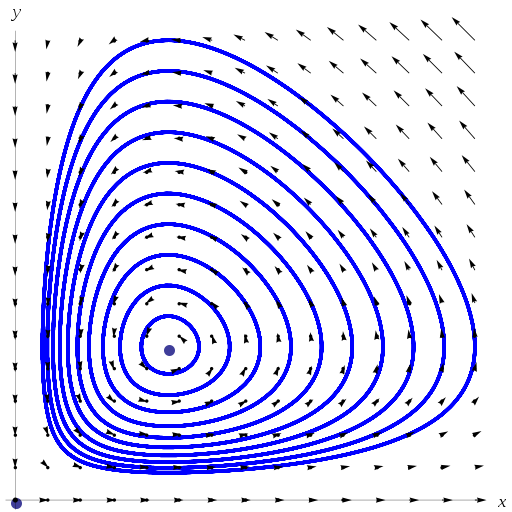
\includegraphics[width=\linewidth]{punto_equilibrio/orbite_sistema_preda_predatore}
					\end{wrapfigure}
					$ P_B $:\\
					Ovunque mettiamo la coppia preda-predatore, essa si trova su un orbita chiusa di $ P_B $.\\
					Allontanandosi dal punto, le orbite si allargano fino a degenerare e a coincidere con gli assi. Quindi si tratta di un punto di equilibrio semplicemente stabile.
				}
		\end{itemize}
	
		\noindent
		Adesso analizziamo il sistema linearizzandolo:
		\[ 
			\pder{f}{x} = 
			\begin{bmatrix}
				r(1-x_2) & -r x_1\\
				d x_2 & d(x_1-1)
			\end{bmatrix}
		\]
		\begin{itemize}
			\item
				attorno $ P_A $: $ \hat A = \left. \pder{f}{x} \right|_{(0,0)} = \begin{smallmatrix} r & 0\\ 0 & -d \end{smallmatrix} $.\\
				Il sistema linearizzato ha un autovalore reale positivo, allora il punto di equilibrio del sistema no lineare \'e instabile.
			\item
				attorno $ P_B $: $ \hat A = \begin{smallmatrix} 0 & -r\\ d & 0 \end{smallmatrix} $
				\[ \phi(s) = det \begin{smallmatrix} s & r\\ -d & s \end{smallmatrix} = s^2 + rd \]
				Poich\'e $ rd > 0 $, abbiamo due radici immaginarie pure con molteplicit\'a $ 1 $: $ s_1 = j\sqrt{rd} $ e $ s_2 = -j\sqrt{rd} $. Il sistema linearizzato \'e semplicemente stabile, ma questo non ci basta per concludere anche per il sistema non lineare.
		\end{itemize}
\end{document}